\subsubsection{Selección de varilla trapezoidal} 
\label{sec:mov_vertical}
El sistema de elevación vertical debe soportar una carga total de 1.2\,kg (lechuga y accesorios) a lo largo de una varilla de 2\,m de longitud. La varilla está fijada por su extremo superior y la carga se desplaza a lo largo de ella mediante una tuerca, trabajando por lo tanto a tracción. Se adopta un factor de seguridad de 4 para contemplar cargas dinámicas, desalineaciones y degradación del sistema con el uso.

Aunque la varilla trabaja principalmente a tracción, es necesario verificar la estabilidad estructural frente a posibles cargas de compresión durante maniobras o situaciones no previstas. Considerando que la varilla tiene ambos extremos empotrados, la carga crítica de Euler se calcula como:

\begin{equation}
P_{\text{cr}} = \frac{\pi^2 \cdot E \cdot I}{(K \cdot L)^2}
\label{eq:euler_pandeo}
\end{equation}

donde:
\begin{itemize}[label=$\bullet$]
    \item $E = 200$\,GPa = 200\,000\,N/mm$^2$ (módulo de Young del acero)
    \item $I$ = momento de inercia de la sección transversal de la varilla
    \item $L = 2\,000$\,mm (longitud de la varilla)
    \item $K = 0.5$ (factor de longitud efectiva para ambos extremos empotrados)
\end{itemize}

La carga admisible debe satisfacer:
\begin{equation}
P_{\text{adm}} = \frac{P_{\text{cr}}}{FS} > W
\end{equation}

donde $W = m \cdot g = 1.2\,\text{kg} \cdot 9.81\,\text{m/s}^2 = 11.77$\,N es el peso a soportar, y $FS = 4$ es el factor de seguridad adoptado.

Por lo tanto:
\[P_{\text{adm}} > 11.77\,\text{N} \cdot 4 = 47.08\,\text{N}\]

\underline{Selección del diámetro}
Tras evaluar diferentes diámetros comerciales de varillas trapezoidales de acero, se selecciona una varilla TR16$\times$8 (diámetro nominal 16\,mm, paso 8\,mm).

Para una varilla de diámetro exterior $d_e = 16$\,mm, el momento de inercia de la sección circular es:
\[I = \frac{\pi \cdot d_e^4}{64} = \frac{\pi \cdot 16^4}{64} = 3\,217\,\text{mm}^4\]

Sustituyendo en la ecuación~(\ref{eq:euler_pandeo}) con $K = 0.5$ para extremos empotrados:
\[P_{\text{cr}} = \frac{\pi^2 \cdot 200\,000\,\text{N/mm}^2 \cdot 3\,217\,\text{mm}^4}{(0.5 \cdot 2\,000\,\text{mm})^2} = \frac{6\,341\,481\,520}{1\,000\,000} = 6\,341\,\text{N}\]

La carga admisible resulta:
\[P_{\text{adm}} = \frac{6\,341\,\text{N}}{4} = 1\,585\,\text{N} > 47.08\,\text{N}\]

Se verifica que la varilla seleccionada cumple ampliamente con los requerimientos de resistencia, proporcionando un margen de seguridad de aproximadamente 33.7 veces la carga mínima requerida, garantizando la integridad estructural del sistema incluso ante condiciones adversas.

\begin{figure}[H]
    \centering
    \begin{subfigure}{0.35\textwidth}
        \centering
        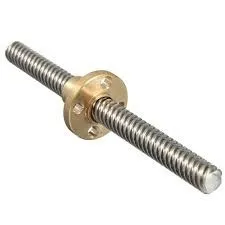
\includegraphics[width=0.7\textwidth]{img/v_roscada.png}
        \caption{\textit{Varilla trapezoidal 16x8.}}
        \label{fig:v_roscada}
    \end{subfigure}
    \hspace{0.5cm}
    \begin{subfigure}{0.35\textwidth}
        \centering
        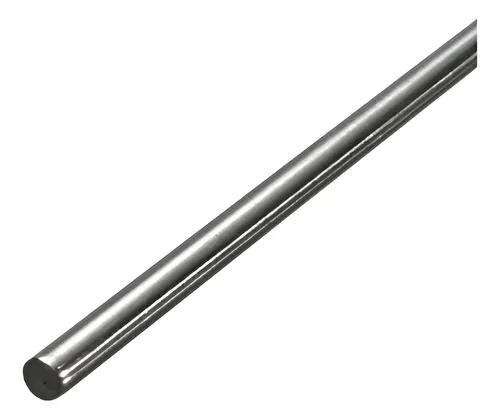
\includegraphics[width=0.7\textwidth]{img/varilla lisa.png}
        \caption{\textit{Varilla de acero maciza de 16mm de diametro.}}
        \label{fig:varilla lisa}
    \end{subfigure}
    \caption{\textit{Sistema de transmisión vertical.}}
\end{figure}

El sistema debe operar con los siguientes parámetros:
\begin{itemize}[label=$\bullet$]
    \item Velocidad lineal máxima: 75\,mm/s
    \item Paso de varilla: 8\,mm
    \item Velocidad angular (pasos completos): $\omega = \frac{v_{\text{lineal}}}{\text{paso}} \cdot 60 = \frac{75\,\text{mm/s}}{8\,\text{mm}} \cdot 60 \approx 562.5$\,rpm
    \item Microstepping: 1/8 paso (1\,600 pasos/revolución)
    \item Resolución: $\frac{1\,600\,\text{pasos/rev}}{8\,\text{mm/rev}} = 200$\,pasos/mm
\end{itemize}

El uso de microstepping 1/8 permite mantener una alta resolución de 200\,pasos/mm (equivalente a 0.005\,mm o 5\,micrones por paso) mientras se opera a baja velocidad, maximizando el torque disponible del motor y proporcionando un movimiento suave y preciso.\\
%\subsubsection{Cálculo de torque y selección del motor}
\subsubsection{Cálculo de torque motor para accionamiento vertical}

El torque requerido para mover una carga mediante una varilla trapezoidal se compone de dos componentes: el torque necesario para vencer la fricción en la rosca y el torque para vencer la fricción en el collarín del soporte. Dicho torque se calcula a partir de la ecuación \ref{eq:torque_total_varilla}

donde:
\begin{itemize}[label=$\bullet$]
    \item $F = 1.2\,\text{kg} \cdot 9.81\,\text{m/s}^2 = 11.77$\,N
    \item $d_m = 14$\,mm
    \item $d_c \approx 26$\,mm
    \item $\mu_c = 0.2$
    \item $k_R = 1.5$ (para paso de 8\,mm, ángulo de hélice $\approx 10.3^\circ$)
    \item $k_L = 0.5$ (para paso de 8\,mm)
\end{itemize}

Sustituyendo valores en las ecuaciones~(\ref{eq:torque_subida}) y~(\ref{eq:torque_bajada}):

\[T_{\text{subida}} = \frac{11.77 \cdot 14}{2} \cdot 1.5 + \frac{11.77 \cdot 0.2 \cdot 26}{2} = 123.6 + 30.6 = 154.2\,\text{Nmm}\]

\[T_{\text{bajada}} = \frac{11.77 \cdot 14}{2} \cdot 0.5 + \frac{11.77 \cdot 0.2 \cdot 26}{2} = 41.2 + 30.6 = 71.8\,\text{Nmm}\]

El torque de diseño se toma como el mayor de ambos:
\[T_{\text{base}} = \max(T_{\text{subida}}, T_{\text{bajada}}) = 154.2\,\text{Nmm} = 0.154\,\text{Nm}\]

Se aplican los siguientes factores correctivos:

\begin{enumerate}
    \item \textbf{Factor por fricción adicional en roscas trapezoidales ($f_1 = 2.0$):} Las roscas trapezoidales presentan pérdidas significativas por fricción que no están completamente capturadas en las ecuaciones simplificadas. Estas pérdidas se deben a:
    \begin{itemize}[label=$\bullet$]
        \item La geometría de los canales trapezoidales, que generan mayor área de contacto y fricción entre los flancos de la rosca y la tuerca
        \item El efecto de acuñamiento de la rosca durante el movimiento, especialmente pronunciado en roscas trapezoidales comparado con roscas de bolas
        \item El roce continuo metal-metal entre la tuerca y toda la longitud de la rosca, que genera calentamiento y puede aumentar la fricción
        \item Pérdidas adicionales por desalineación a lo largo de los 2\,m de varilla
        \item Variaciones en la calidad de la lubricación durante la vida útil del sistema
    \end{itemize}
    El paso de 8\,mm reduce este factor respecto a pasos menores debido a la menor cantidad de vueltas necesarias para el mismo desplazamiento lineal, disminuyendo las pérdidas acumulativas por fricción.

    \item \textbf{Factor de seguridad por caída de torque con velocidad ($f_2 = 1.2$):} Los motores paso a paso experimentan una reducción significativa del torque disponible al aumentar la velocidad de rotación, como se observa en las curvas dinámicas. Dado que el sistema opera a baja velocidad (70.3\,rpm), el motor mantiene la mayor parte de su torque nominal, requiriendo un factor de seguridad menor.
\end{enumerate}

El torque motor requerido resulta:
\begin{equation}
T_{\text{motor}} = T_{\text{base}} \cdot f_1 \cdot f_2 = 0.154 \cdot 2.0 \cdot 1.2 = 0.37\,\text{Nm}
\label{eq:torque_motor_vertical}
\end{equation}

\subsubsection{Selección del motor paso a paso}
Considerando la velocidad de operación de 70.3\,rpm (con microstepping 1/8), se verifica en la curva dinámica torque-velocidad (Figura~\ref{fig:Curva_din_nema34}) que se requiere un torque disponible de al menos 0.37\,Nm.

Se selecciona un motor \textbf{NEMA 34 Medium} con las siguientes especificaciones:
\begin{itemize}[label=$\bullet$]
    \item Alimentación: 24\,V / 4.5\,A
    \item Torque de retención (holding torque): $>$ 3\,Nm
    \item Torque a 70.3\,rpm: $\approx$ 2.5\,Nm (según curva dinámica)
\end{itemize}

El motor seleccionado proporciona un margen de seguridad de aproximadamente 6.76 veces el torque requerido a la velocidad de operación, garantizando movimientos suaves y seguros durante toda la operación del sistema, incluyendo situaciones de carga máxima y fricción elevada. La baja velocidad de operación permite aprovechar el torque máximo disponible del motor, resultando en un diseño robusto y confiable.

\begin{figure}[H]
    \centering
    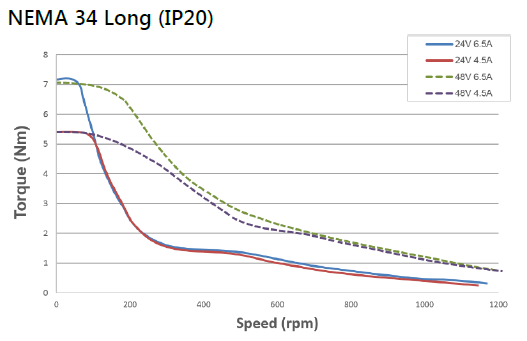
\includegraphics[width=0.65\textwidth]{img/Nema34.png}
    \caption{\textit{Curva dinámica torque-velocidad del motor paso a paso NEMA 34 Medium. Se observa que a 70.3\,rpm el torque disponible es de aproximadamente 2.5\,Nm, superando ampliamente el requerimiento calculado de 0.37\,Nm con un margen de seguridad de 6.76 veces.}}
    \label{fig:Curva_din_nema34}
\end{figure}